\chapter{Antennen}
\lit{Kurzwellen-Drahtantennen Praktikum von Max Rüegger, HB9ACC. Quelle: htc.ch}

\section{Dipol}
Ein Dipol besteht grundsätzlich aus zwei gestreckten Antennendrähten, die zusammen die Länge $\lambda/2$ (oder ein ganzzahliges Vielfaches davon) ergeben. Sie werden mittig mit hochfrequentem Wechselstrom gespiesen. Der Dipol kann auf der Grundfrequenz und auf ganzzahligen Vielfachen davon betrieben werden.

Neben dem offenen Dipol (Impedanz 50–75 Ohm) existieren noch weitere Varianten wie die \textit{Inverted Vee}, die von einem Antennenmast auf beide Seiten heruntergespannt wird, und verschieden geformte Loops wie der breitbandigere Faltdipol oder der Quad Loop. Loops \textit{(Schleifenantennen)} haben eine höhere Impedanz (240–300 Ohm) und werden aus einem $\lambda$ langen Antennenkabel geformt.

Beim Loop gilt: Je grösser die von der Antenne überdeckte Fläche, desto besser.

\section{Longwire}
Einfache Kabel, die am Ende gespiesen werden (und nicht mittig wie der Dipol). Diese hochomigen Antennen benötigen eine Erdung als Gegengewicht und eine symmetrische Speiseleitung (zum Beispiel eine sogenannte Hühnerleiter). 

\section{Groundplane}
Die Groundplane-Antenne besteht aus einem Strahler und einem Gegengewicht. Der vertikale Strahler wird in Längen von $\lambda/2$, $\lambda/4$ und $\frac{5}{8}\,\lambda$ gebaut. Die $\frac{5}{8}\,\lambda$ eignet sich aufgrund des flacheren Abstrahlwinkels gut für DX-Verbindungen, während die  $\lambda/4$ einen steilen Abstrahlwinkel aufweist.

Als Gegengewicht verwendet man sogenannte Radials (da sie radial von der Antenne weggehen) mit der Länge des Strahlers. Je nachdem werden sie in die Erde vergraben oder über dem Boden gespannt. Werden sie ungefähr einen Meter über dem Boden gehalten, kann der Gewinn unter Umständen um 3 S-Stufen steigen.

Die Impedanz beträgt 36 Ohm, kann aber mit den Radials verändert werden (etwa auf 50 Ohm).

Für mobile VHF/UHF-Antennen kann z.\,B. das Auto als Gegengewicht verwendet werden.

\section{Logper}
Da sie sich auf verschiedenen Bändern einsetzen lassen, wird die Logper-Antenne (auch LPDA, Logarithmic-Periodic Dipole Array, genannt) immer beliebter. Sie ist aus unterschiedlich grossen, gegengleich verdrahteten Dipolen aufgebaut. Beim Senden sucht sich jede Frequenz den passenden Dipol; das vordere Element wirkt als Direktor und das hintere als Reflektor. So sind immer ungefähr drei bis vier Elemente aktiv. Eine Logper ist somit aus der Sicht einer Frequenz eine Dreielement-Antenne und weist auch einen ähnlichen Gewinn auf.

\begin{figure}[h!]
 \centering
 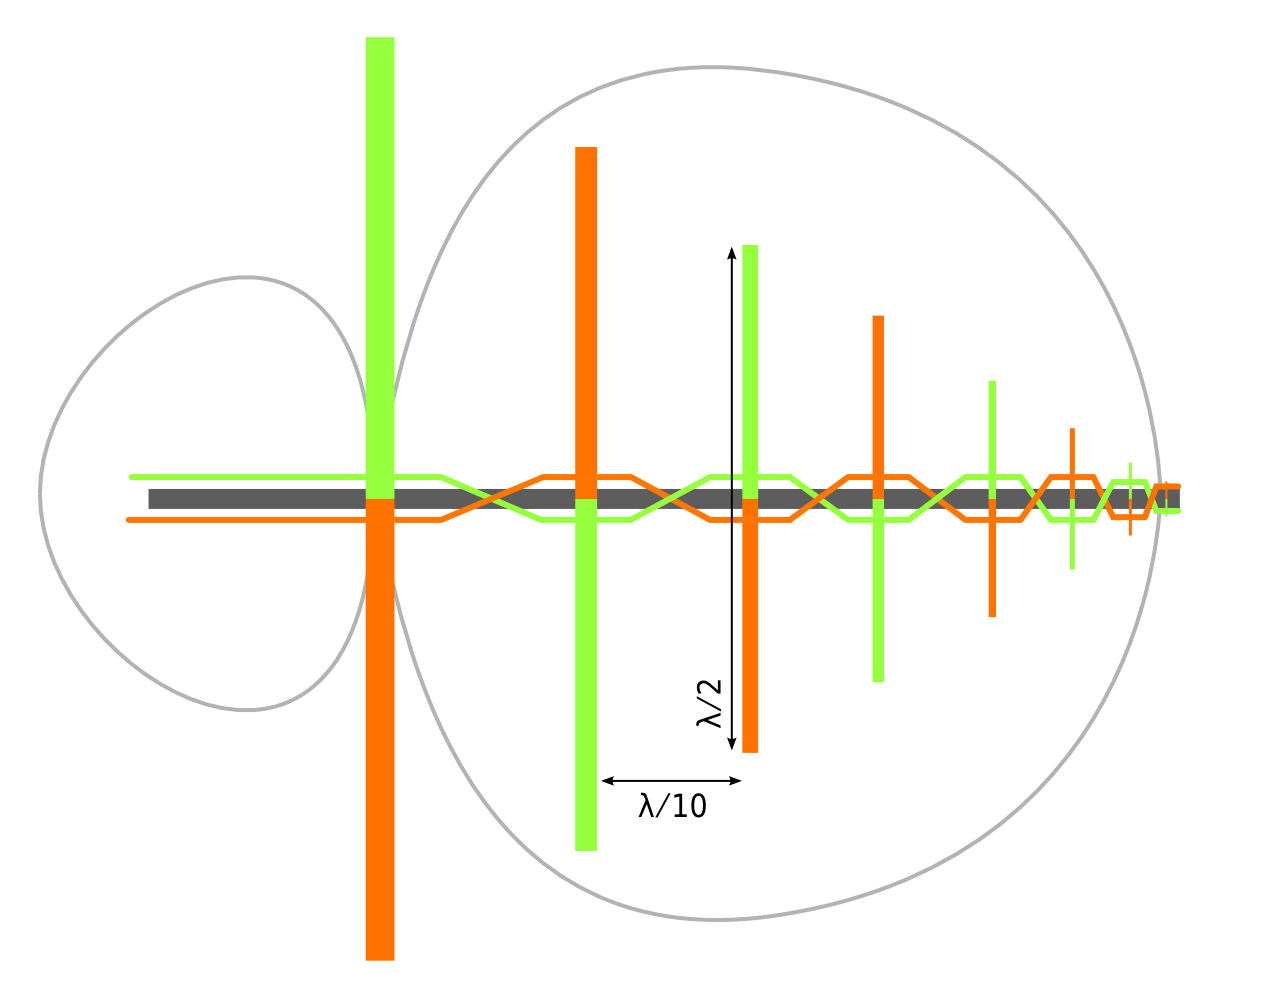
\includegraphics[width=6cm]{./png/Amfu-Logper.png}
 \caption{Aufbau, Stromverteilung und Abstrahldiagramm einer Logper.}
 \label{fig:logper}
\end{figure}

Für einen besseren Gewinn oder eine grössere Bandbreite muss die Logper länger sein. Aufgrund der Grösse wird sie im Amateurfunk praktisch nur für VHF/UHF eingesetzt, bei militärischen Einrichtungen sind auch Logper-Antennen für HF zu sehen.

\section{Yagi}
Yagis (eigentlich Yagi-Uda-Array; erfunden wurde sie vom Japaner Uda, Yagi übersetzte den Artikel nur zuerst nach Englisch) oder \textit{Beams} werden vor allem im Bereich VHF/UHF verwendet. Sie sind eher schmalbandige Richtstrahlantennen und bestehen aus einem Strahler – ein einfacher Dipol –, einem Reflektor und aus mindestens einem Direktor. Die Direktoren, die in die gewünschte Abstrahlrichtung zeigen, sind etwa $0.05 \lambda$ kürzer, der Reflektor auf der anderen Seite ungefähr $0.05 \lambda$ länger. Ein dreielementiges Yagi hat einen Gewinn von etwa 5 dB, mit weiteren Elementen sind bis 20 dB erreichbar.

\begin{figure}[h!]
 \centering
 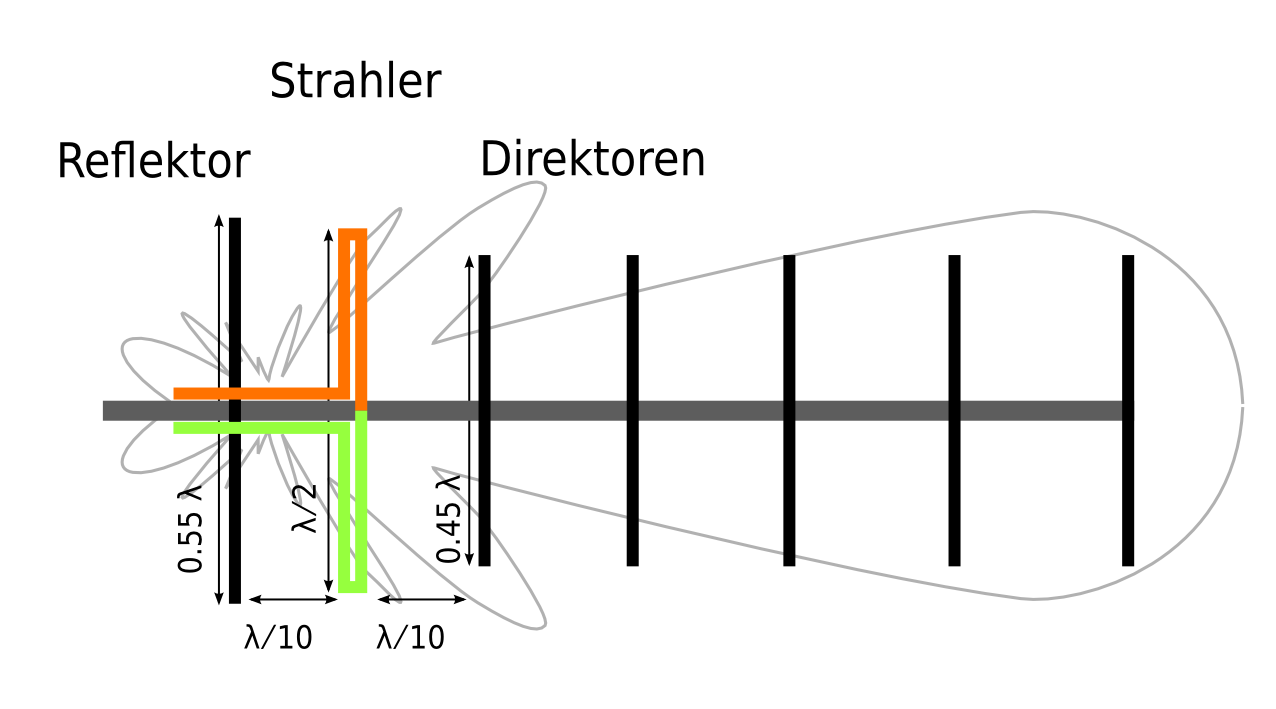
\includegraphics[width=6cm]{./png/Amfu-Yagi.png}
 \caption{Aufbau, Stromverteilung und Strahlungsdiagramm einer Yagi.}
 \label{fig:yagi}
\end{figure}

Auf älteren Hausdächern sieht man teilweise noch Yagis für den Fernsehempfang.

Mit Yagis kann man aufgrund der Richtwirkung in eine bestimmte Richtung besser senden und empfangen. 

\section{Magnetantenne}
Anders als herkömmliche Antennen arbeitet die Magnetantenne mit dem magnetischen Anteil des elektromagnetischen Signals. Sie lässt sich mit Durchmessern um einen Meter sehr platzsparend bauen und eignet sich daher gut für dicht besiedelte Gebiete. Ein Nachteil ist jedoch, dass sie sehr schmalbandig ist und sogar bei Frequenzwechseln innerhalb eines Bandes nachgestellt werden muss.

Ab einem Umfang von mehr als $\lambda∕10$ spricht man wieder von einer elektromagnetischen Antenne, da der elektrische Teil dann wieder zunimmt.



